\section{Dataset-Level Effect of the Deployment Rule}
Table~\ref{tab:dcd_ablation} reports the macro effect of replacing
gating+fusion with the fixed candidate.  Figure~\ref{fig:dcd_deployment}
shows the per-dataset trade-off.  DCD improves both Dice and HD95 on two
datasets, improves Dice but degrades HD95 on six, improves HD95 but degrades
Dice on two, and degrades both on two.  The large HD95 gain on TopoMortar
(+24.1 px) contrasts with HD95 losses on most other datasets, which is why
we do not claim uniform superiority.

\begin{figure*}[t]
\centering
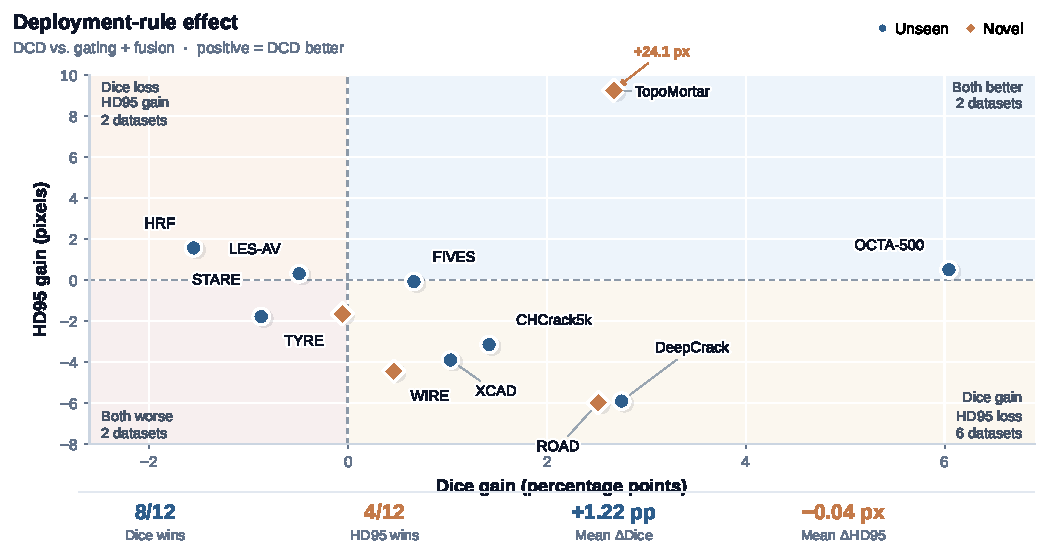
\includegraphics[width=\textwidth]{../figures/fig4_deployment_scatter.pdf}
\caption{Dataset-level trade-off of the deterministic deployment rule.
Each point is one of the 12 evaluation datasets; the horizontal axis is the
Dice gain of DCD (fixed candidate 3) over gating+fusion, and the vertical
axis is the HD95 gain.  Positive values indicate DCD is better.  Blue
circles and orange diamonds denote Unseen and Novel datasets, respectively.
The four quadrants contain datasets where DCD improves both metrics (2),
only Dice (6), only HD95 (2), or neither (2).  The HD95 gain of TopoMortar
(+24.1 px) is clipped and marked with an arrow.  Values are four-seed
means.}
\label{fig:dcd_deployment}
\end{figure*}
